\section{Problem (5)}
	The body in \cref{fig:hwa_problem5} is pivoted at $O$. Three forces act on it in the directions shown: $F_{A} = \ 9.3 \ N$ at point $A$, $7.5 \ m$ from $O$; $F_{B} = \ 11.0 \ N$ at point $B$, $5.4 \ m$ from $O$; and $F_{C} = \ 8.8 \ N$ at point $C$, $4.4 \ m$ from $O$. Taking the clockwise direction to be negative, what is the net torque about $O$?

	\begin{figure}[H]
		\begin{center}
			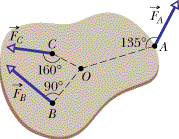
\includegraphics[scale=1]{hwa_problem5}
			\caption{Illustration of Problem 5}
			\label{fig:hwa_problem5}
		\end{center}
	\end{figure}

	\textbf{R:}

	\begin{align}
		\tau_{A} = \ &r_{A\perp}F_{A}& \notag \\
		= \ &(7.5 \ m)(9.3 \ N) \sin 45^{o}& \notag \\
		= \ &49.321 \ N \times m& \notag \\
		\tau_{B} = &r_{B\perp}F_{B}& \notag \\
		= \ &-(4.4 \ m)(8.8 \ N) \sin 90^{o}& \notag \\
		= \ &-38.720 \ N \times m& \notag \\
		\tau_{C} = &r_{C\perp}F_{C}& \notag \\
		= \ &(5.4 \ m)(11.0 \ N) \sin 30^{o}& \notag \\
		= \ &29.700 \ N \times m& \notag \\
		\tau_{net} = &\tau_{A} + \tau_{B} + \tau_{C}& \notag \\
		= \ &(49.321 \ N \times m) + (-38.720 \ N \times m) + (29.700 \ N \times m)& \notag \\
		= \ &(49.321 \ N \times m) + (-38.720 \ N \times m) + (29.700 \ N \times m)& \notag \\
		= \ &40.301 \ N \times m&
	\end{align}
